\documentclass[10pt,aspectratio=169]{beamer}

\usetheme[progressbar=frametitle]{metropolis}
\usepackage{appendixnumberbeamer}

\usepackage{booktabs}
\usepackage[scale=2]{ccicons}

\usepackage{pgfplots}
\usepgfplotslibrary{dateplot}

\usepackage{xspace}
\newcommand{\themename}{\textbf{\textsc{metropolis}}\xspace}

\usepackage[default]{lato}

\title{Protocolo de Tesis}
\subtitle{Cuantificación de incertidumbre bayesiana aproximada en problemas inversos de ODE}
% \date{\today}
\date{}
\author{César Isaí García Cornejo\\
Asesor: Dr. José Andrés Christen Gracia}
\institute{CIMAT}
% \titlegraphic{\hfill\includegraphics[height=1.5cm]{logo.pdf}}
% ////////////////////////////////////////////////////////////
% ////////////////////////////////////////////////////////////
\begin{document}

\maketitle

% \begin{frame}{Table of contents}
%   \setbeamertemplate{section in toc}[sections numbered]
%   \tableofcontents%[hideallsubsections]
% \end{frame}

\section[Introducción]{Introducción}

\begin{frame}[fragile]{Introducción}
  
  Los modelos que pretendan describir los fenómenos naturales deben ser causales, respetando orden entre causa y efecto.

  Típicamente, los modelos matemáticos precisan de condiciones iniciales o parámetros  para caracterizar la unicidad en su solución. Tales parámetros se conocen como parámetros del modelo y se interpretan como causas del fenómeno modelado. Mientras que la solución del modelo se interpreta como la predicción del fenómeno, que se asocia a los efectos.
  
\end{frame}


\begin{frame}[fragile]{Introducción}
  
  El proceso anteriormente descrito se llama problema directo o \textit{forward problem} ya que sigue la dirección de causalidad. Sin embargo, es interesante también el problema inverso, dada ciertas observaciones de las cualidades de un fenómeno (efectos), \textbf{¿es posible calcular las causas del modelo que rige el fenómeno?}

  % \begin{figure}[H] 
  %     \centering 
  %     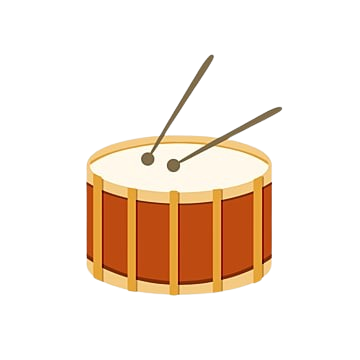
\includegraphics[width = 4 cm]{Figures/tambor2.png} 
  %     % \caption{}
  %     % \label{Fig. }
  % \end{figure} 

\end{frame}


\begin{frame}[fragile]{Sistema físico}

  \textbf{Estudio de un sistema físico:}
  \begin{figure}[H] 
      \centering 
      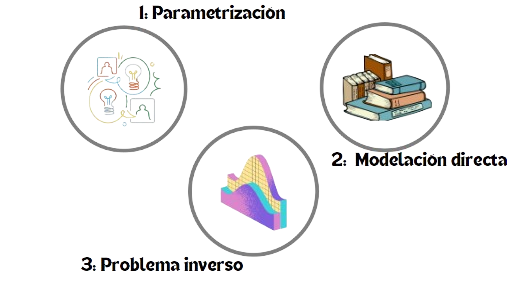
\includegraphics[width = 10 cm]{Figures/Modelos.png} 
      % \caption{}
      % \label{Fig. }
  \end{figure} 
  % \begin{enumerate}
  %     \item Parametrización del sistema: descubrimiento del conjunto mínimo de parámetros del modelo cuyos valores caracterizan completamente el sistema.
  %     \item Modelación directa (forward modeling): Descubrimiento de las leyes físicas que nos permiten hacer predicciones, dado valores de parámetros del modelo, de mediciones en observables físicas.
  %     \item Modelación inversa: Usar las mediciones de las observables físicas para inferir los valores de los parámetros del modelo.
  % \end{enumerate}

  % Los experimentos sugieren teorías físicas, y las teorías físicas predicen los resultados de los experimentos. La comparación entre la predicción y las observaciones son evidencia de la factibilidad de la teoría.
\end{frame}


\section{Antecedentes}

\begin{frame}{Modelos Descritos por ODEs}
  Consideramos modelos de la forma
  \begin{align*}
    G(t,y(t),y'(t),y''(t),...) = 0
  \end{align*}
  con $y(0)=y_0, y'(0)= y'_0, \cdots$ sus condiciones iniciales.

  Más aún, se puede generalizar a sistemas de ecuaciones diferenciales (Apostol, 2019).
\end{frame}


\begin{frame}{Forward Map}
  El \textbf{problema directo} es entonces aquel que dado un $\theta \in \Theta$ obtiene la trayectoria o solución de la ecuación diferencial.

  \vspace{1 cm}
  
  Denotemos por $\mathcal{Y}$ al espacio de las soluciones posibles de la ecuación diferencial. De esta forma existe un mapeo del espacio $\Theta$ a $\mathcal{Y}$ el cual llamaremos \textbf{forward map}. Así, el forward map es 
  \begin{align*}
      \theta \mapsto F[\theta]
  \end{align*}
  donde $\theta \in \Theta$ y $F[\theta] \in \mathcal{Y}$.
\end{frame}

\begin{frame}{Problema Inverso}
  Ejemplo
  
\end{frame}

\begin{frame}{Solución Bayesiana al Problema Inverso}
  Principalmente existen dos razones para que las observaciones de un modelo no concuerden exactamente con las predicciones.

  \begin{enumerate}
    \item Errores de medición por la incertidumbre de los aparatos de medición.
    \item Defectos propios del modelo.
  \end{enumerate}
\end{frame}

\begin{frame}
  El paradigma bayesiano para problemas inversos se centra en cuantificar la incertidumbre en los parámetros del modelo.Es decir, su objetivo es establecer una medida de probabilidad posterior a las observaciones de la trayectoria del modelo. Equivalentemente, se busca la distribución de probabilidad $\pi(\theta|\mathbf{y})$ donde $\mathbf{y} = (y_1,...,y_n)$ son las observaciones de la trayectoria a lo largo del tiempo $t_1, t_2, \cdots, t_n$. Partiendo de la información acerca de los parámetros previo a cualquier observación, se propone una distribución de probabilidad $\pi(\theta)$ llamada distribución a priori, y tras aplicar el Teorema de Bayes obtener la distribución posterior (Wasserman,2013).
\end{frame}

\begin{frame}{Cuantificación de la Incertidumbre}
  De esta forma, se establece que las discordancias entre observaciones y predicciones siguen una distribución normal de la forma
  \begin{align*}
      y_i = F_{\theta} (t_i) + \varepsilon_i, \:\:\:\:\:\: \varepsilon_i \sim N(0,\sigma^2),
  \end{align*}
  donde las $y_i's$ son las observaciones del fenómeno.
\end{frame}

\begin{frame}{Distribución Posterior}
  Se ha establecido una distribución para las observaciones $y_i$ las cuales tienen asociada una verosimilitud sobre $\theta$ y $\sigma$. Como se consideran errores condicionalmente independientes, pues se tratan de errores de medición, la verosimilitud se sigue de
  \begin{align*}
      \mathcal{L}(\theta,\sigma) &= f(\mathbf{y}|\theta,\sigma) = \prod_{i = 1}^{n} \frac{1}{\sqrt{2\pi \sigma^2}} \exp \left \{ -\frac{1}{2\sigma^2}\left(y_i - F_{\theta}(t_i)\right)^2 \right \} , 
  \end{align*}
  simplificando
  \begin{align}
      f(\mathbf{y}|\theta,\sigma) = \left(\frac{1}{2\pi \sigma^2}\right) ^{n/2}\exp \left \{  -\frac{1}{2\sigma^2}\sum_{i = 1}^{n} \left(y_i - F_{\theta}(t_i)\right)^2 \right \},
      \label{2.2.03}
  \end{align}
\end{frame}


\begin{frame}{Distribución Posterior} 
  Del teorema de Bayes, se obtiene la distribución posterior para los parámetros
  \begin{align}
      \pi(\theta,\sigma | \mathbf{y})  = \frac{f(\mathbf{y}|\theta)\pi(\theta)}{\int f(\mathbf{y}|\theta)\pi(\theta)d \theta}.
      \label{2.2.04}
  \end{align}
  donde la constante de integración $h(\mathbf{y}) = \int f(\mathbf{y}|\theta)\pi(\theta)d \theta$ es la constante de normalización para la distribución posterior. 
\end{frame}

\begin{frame}{Método MCMC}
  Simulación de la posterior. $1/\sqrt{n}$
\end{frame}


\begin{frame}{Algoritmo de Metropolis-Hastings} 
  El algoritmo de Metropolis-Hastings es un método de MCMC para generar muestras de una distribución objetivo $f(x)$ partiendo de muestras de una distribución propuesta $q(y|x)$.

  el algoritmo de Metropolis-Hastings genera una cadena $X_0, X_1, \cdots, X_N$ construyendo recursivamente la cadena dependiendo solamente del estado previo, es decir preservando la propiedad de Markov.
\end{frame}




























\begin{frame}{Algoritmo de Metropolis-Hastings}
  El estado inicial $X_0$ se toma aleatoriamente. Luego, teniendo hasta el estado $X_i$, el estado $X_{i+1}$ se obtiene siguiendo 
  \begin{enumerate}
      \item Generar una propuesta $Y \sim q(y|X_i)$.
      \item Calcular $\rho$ 
      \begin{align*}
          \rho = \min \left \{ \frac{f(y)q(x|y)}{f(x)q(y|x)}, 1  \right \} 
      \end{align*}
      \item Realizar un experimento Bernoulli con probabilidad de éxito $\rho$.
      \begin{align*}
          X_{i+1} = \left\{\begin{matrix}
          Y & , \:\:\: \text{con probabilidad} \:\:\:\:\: \rho  \\ 
              X_{i}&,  \text{con probabilidad} \:\:\:\:\: 1- \rho  
            \end{matrix}\right.
      \end{align*}
  \end{enumerate}
\end{frame}

\begin{frame}{Algoritmo de Metropolis-Hastings}
  \begin{figure}[H] 
    \centering 
    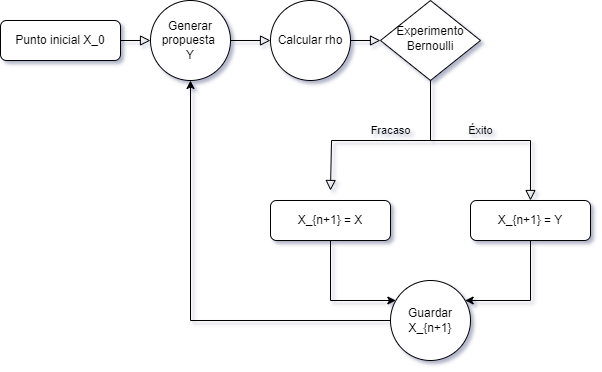
\includegraphics[width = 12 cm]{img/MCMC.png} 
    % \caption{}
    \label{Fig. M-H}
  \end{figure} 
\end{frame}

\begin{frame}
  Explicación punto por punto de M-H.
\end{frame}

\begin{frame}{Forward Map Aproximado}
  
  \begin{itemize}
    \item 
    El forward map aproximado $F_{\theta}^{*}$ es una construcción multifacética basada en aproximaciones de estadística espacial. 
    \vspace{0.5 cm}
    \item
    Tal aproximación pretende crear una distribución posterior aproximada $\tilde{\pi}(\theta|\mathbf{y})$ con la sustitución del forward map a su versión aproximada.
    \item 
    \vspace{0.5 cm}
    Existen diferentes maneras de hacer las aproximaciones del forward map. La forma propuesta es considerar una discretización del espacio de parámetros $\Theta$.
  \end{itemize}
  



\end{frame}

\begin{frame}{Construcción del Forward Map Aproximado}

  Para cada $\theta \in \Theta \subset \mathbb{R}^d$ se puede escribir como $\theta = (\theta_1, \theta_2, \cdots, \theta_d)$.

  Consideremos para cada coordenada un intervalo $[\theta_i^{min},\theta_i^{max}]$ para toda $i \in \{1,\cdots,d\}$, donde $\theta_i^{min}$ y $\theta_i^{max}$ son cotas para el espacio de parámetros que contenga la masa de probabilidad.
  
  Tomemos una partición equidistante en $M$ puntos para cada coordenada. La partición de la coordenada $i-$ésima es el conjunto $\mathcal{M}_i =\{ \theta_i^{(1)}, \theta_i^{(2)},\cdots , \theta_i^{(M-1)}, \theta_i^{(M)}\}$ con $\theta_i^{(1)} = \theta_i^{min}$ y $\theta_i^{(M)} = \theta_i^{max}$.

  De esta forma, la partición crea una malla $\mathcal{M} = \mathcal{M}_1 \times \cdots \times \mathcal{M}_d$ del espacio parametral $\Theta$.

\end{frame}

\begin{frame}{Construcción del Forward Map Aproximado}
  Sea $\vartheta \in \mathcal{M} $ elemento de la malla $\mathcal{M}$. El forward map para cada elemento de $\mathcal{M}$ es, 
  \begin{align*}
    y_j = F[\vartheta_j],
  \end{align*}
  con $y_j = y_j(t)$ funciones continuas
  
  
\end{frame}

\begin{frame}{Construcción del Forward Map Aproximado}
  Para parámetros $\theta \notin \mathcal{M}$ se propone buscar a los $k$ vectores de parámetros $\vartheta \in \mathcal{M}$ más cercanos en distancia euclidiana a $\theta$, denotando estos $k$ vecinos por $\vartheta^{(1)}, \cdots, \vartheta^{(k)}$ cada uno a una distancia $d_1, \cdots, d_k$ de $\theta$, respectivamente; con $d_1 \leq d_2 \leq \dots \leq d_k$. 
  
  \vspace{0.5 cm}

  La aproximación al forward map con $k$ vecinos en una malla con $M$ particiones es
  \begin{align}
    \tilde{F}^{k}_M(\theta) = \sum_{j = 1}^{k} \omega_j(\theta) F \left(\vartheta^{(j)}\right)
    \label{2.4.01}
  \end{align}
  donde $\omega_j(\theta) = d_j^{-1}/ \sum_{i=1}^{k} d_i^{-1}$
\end{frame}

\begin{frame}{Consistencia y Utilidad del Forward Map Aproximado}
  
\end{frame}





















\begin{frame}
  
\end{frame}

\begin{frame}
  
\end{frame}

\begin{frame}
  
\end{frame}












\begin{frame}[fragile]{Forward map}
  
  \textbf{El problema directo:}
  
  Predecir los valores de las observables físicos $\mathbf{d}$ que corresponde a un modelo $\boldsymbol{\theta}$
  \begin{align*}
      \boldsymbol{\theta} \:\:\:\:\: \mapsto \:\:\:\:\: \mathbf{d} = \mathbf{F(\boldsymbol{\theta})}
  \end{align*}


  \vspace*{1 cm}

  Incertidumbre de las mediciones e imperfecciones del modelo \cite{tarantola2005inverse}. 

\end{frame}


\begin{frame}{Ejemplos}
  \begin{columns}[T,onlytextwidth]
    \column{0.5\textwidth}

    
    \begin{alertblock}{Resorte sujeto a fricción}
      Sea $x(t)$ la posición
      \begin{align*}
        m\ddot{x} = -kx + b \dot{x}
      \end{align*}
    \end{alertblock}
    
    \begin{block}{Caída sujeto a fricción}
      Sea $x(t)$ la posición
      \begin{align*}
        m\ddot{x} = g - b \dot{x}
      \end{align*}
          % $x(0) = \dot{x(0)} = 0$.
    \end{block}

      \begin{alertblock}{Crecimiento poblacional}
        Sea $P(t)$ el tamaño de población
        \begin{align*}
          \frac{dP}{dt} = r P \left(1 - \frac{P}{K}\right) 
        \end{align*}
      \end{alertblock}

    \column{0.5\textwidth}

      \metroset{block=fill}

      \begin{alertblock}{Forward map}
        $\theta = (k,b)  \:\:\: \mapsto \:\:\: F(\theta) = x(t)$
      \end{alertblock}
      
      \vspace*{1 cm}
      
      \begin{block}{Forward map}
        $\theta = (g,b)  \:\:\: \mapsto \:\:\: F(\theta) = x(t)$
      \end{block}

      \vspace*{1 cm}

      \begin{alertblock}{Forward map}
        $\theta = (r,K)  \:\:\: \mapsto \:\:\: F(\theta) = P(t)$
      \end{alertblock}

  \end{columns}
\end{frame}

\begin{frame}[fragile]{Estadística bayesiana}
  
  La distribución posterior 
  \begin{align*}
      \pi(\theta|x^n) &\propto \mathcal{L}(\theta|x^n) \pi(\theta)
  \end{align*}
  

\begin{figure}[H] 
    \centering 
    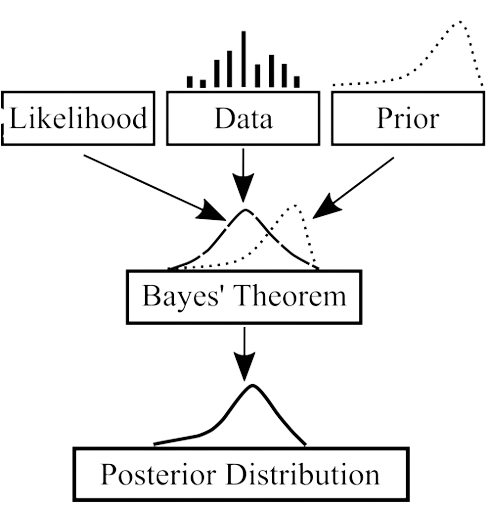
\includegraphics[width = 5.50 cm]{Figures/bayes1.png} 
    % \caption{}
    % \label{Fig. }
\end{figure} 




\end{frame}

\begin{frame}[fragile]{Incertidumbre en los errores}
  Procedimiento:
  \begin{itemize}
    \item 
    \textbf{Observaciones:} $(x_1, t_1), (x_2,t_2), \cdots, (x_n, t_n)$ 
    \item 
    Cuantificar el error mediante la relación
    \begin{align*}
        x_i = F_\theta (t_i) + \varepsilon_i, \:\:\:\:\: i = 1,...,n
    \end{align*}
    \item Un supuesto convencional sobre los errores
    \begin{align*}
        \varepsilon_i \sim N(0,\sigma^2)
        \label{3.02}
    \end{align*}

  \end{itemize}

\end{frame}

\begin{frame}[fragile]{Inferencia}
  
  Distribución posterior 
  \begin{align*}
      \pi(\theta|x^n) &\propto \mathcal{L}(\theta|x^n) \pi_{\Theta}(\theta)\\
      & \left[\propto \prod_{i=1}^n \frac{1}{\sqrt{2\pi \sigma^2}} exp \left({-\frac{1}{2\sigma^2}\left(x_i - F_{\theta}(t_i)\right)^2 }\right)\right] \pi_{\Theta}(\theta) \\
      & \propto \left(\frac{1}{2\pi\sigma^2}\right)^{n/2} exp {\left(\frac{1}{2\sigma^2} \sum_{i =1}^{n}\left(x_i - F_{\theta}(t_i)\right) ^2\right) } \pi_{\Theta}(\theta)
  \end{align*}
  donde $\theta = (\theta_1, ..., \theta_m)$.
  
  \vspace{1 cm}

  \textbf{Simular por métodos Monte Carlo}
  \begin{itemize}
    \item 
    Se simula por MCMC Metropolis-Hastings \cite{robert1999monte}.
  \end{itemize}


  % Es posible simular variables aleatorias con dicha distribución y así obtener estimaciones de los parámetros del modelo.
\end{frame}




\section{Ejemplo}


\begin{frame}{Resorte sujeto a fricción}
  \begin{figure}
      \centering 
      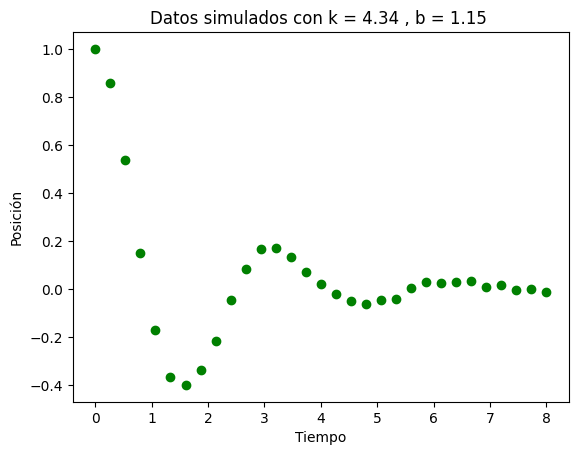
\includegraphics[width = 10cm]{Figures/0.png} 
      % \caption{}
      % \label{Fig. }
  \end{figure} 
\end{frame}

\begin{frame}
  \begin{figure}
      \centering 
      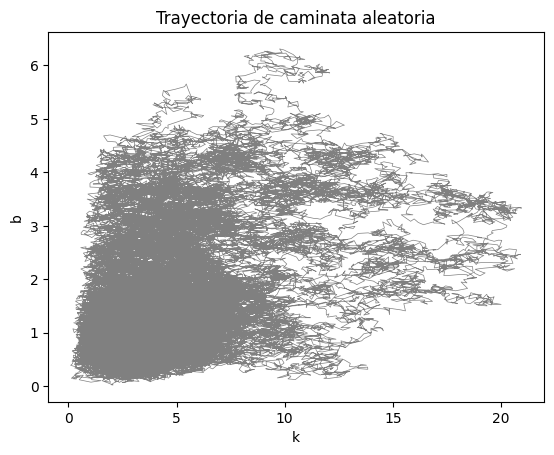
\includegraphics[width = 10 cm]{Figures/1.png} 
      % \caption{}
      % \label{Fig. }
  \end{figure} 
\end{frame}

\begin{frame}
  \begin{figure}[H] 
      \centering 
      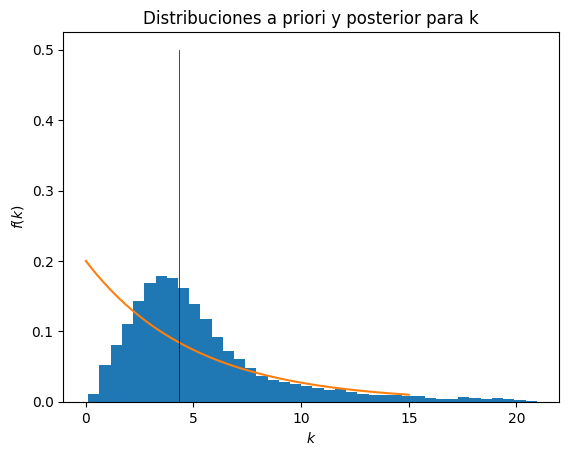
\includegraphics[width = 10 cm]{Figures/2.png} 
      % \caption{}
      % \label{Fig. }
  \end{figure} 
\end{frame}

\begin{frame}
  \begin{figure}[H] 
      \centering 
      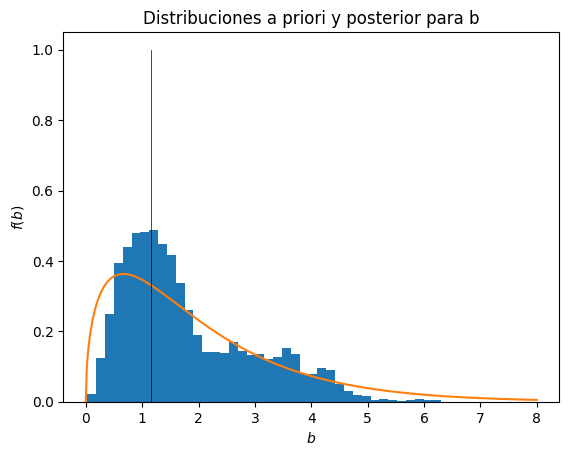
\includegraphics[width = 10 cm]{Figures/3.png} 
      % \caption{}
      % \label{Fig. }
  \end{figure} 
\end{frame}


\begin{frame}
  \begin{figure}[H] 
      \centering 
      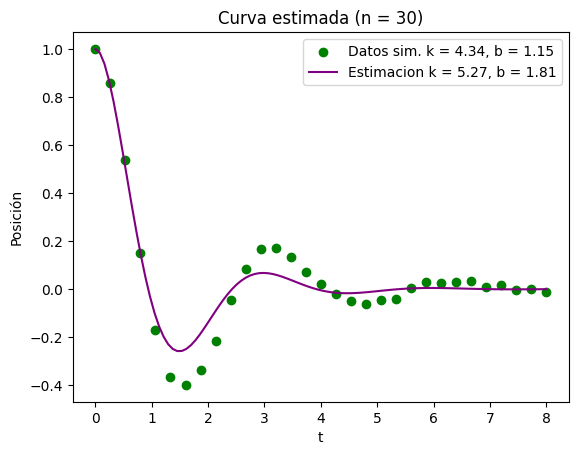
\includegraphics[width = 10 cm]{Figures/4.png} 
      % \caption{}
      % \label{Fig. }
  \end{figure} 
\end{frame}



\section{Objetivos}


\begin{frame}{Objetivos}
  A pesar de que el análisis previo nos permite obtener estimaciones bastante precisas para el problema inverso. Sin embargo, son \textbf{computacionalmente pesadas}, esto debido a que a cada paso en la cadena requiere que se solucione el problema forward, es decir, se resuelven ecuaciones diferenciales tantas veces como se deje correr la cadena. 
  \begin{itemize}
    \item 
    Se desea encontrar una especie de \textit{interpolación} para solo solucionar una cantidad pequeña de veces el problema forward y para cada punto en el espacio de parámetros se pueda aproximar la solución en función de las soluciones con parámetros cercanos.
  \end{itemize}

\end{frame}

\begin{frame}
  \begin{figure}[H] 
      \centering 
      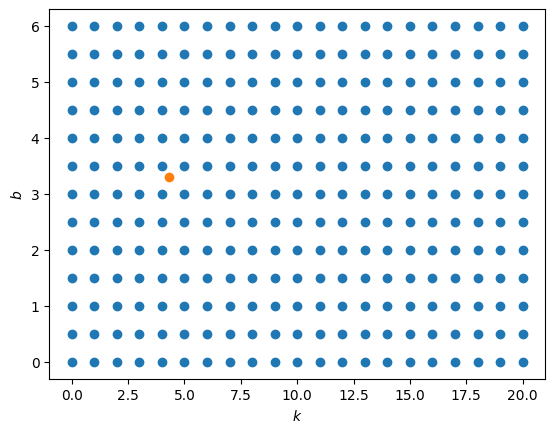
\includegraphics[width = 10 cm]{Figures/5.png} 
      % \caption{}
      % \label{Fig. }
  \end{figure} 
\end{frame}











\section{Plan de trabajo}

\begin{frame}{Plan de trabajo}
  
  \begin{figure}[H] 
      \centering 
      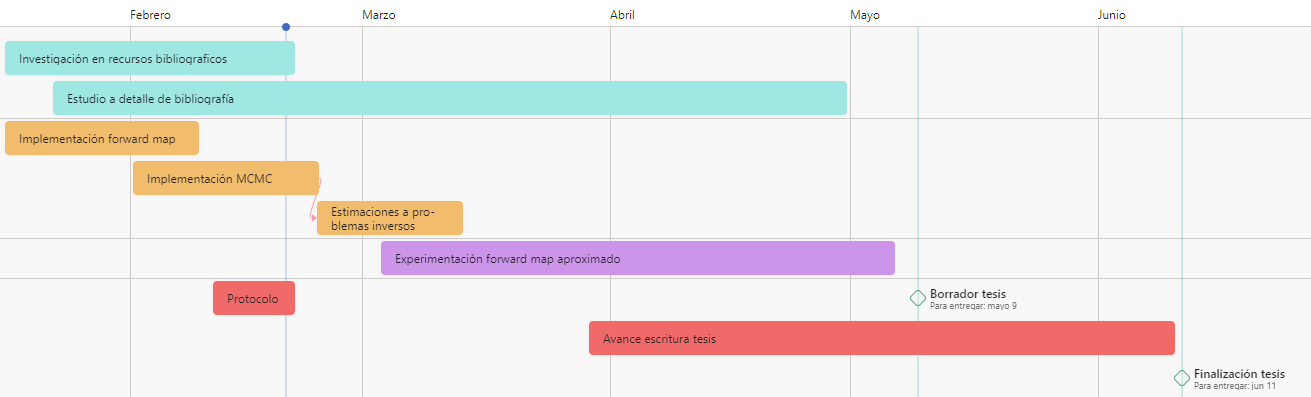
\includegraphics[width = 14 cm]{Figures/cronograma.png} 
      % \caption{}
      % \label{Fig. }
  \end{figure} 
\end{frame}



\begin{frame}{Referencias}

  \bibliography{demo}
  \bibliographystyle{abbrv}

\end{frame}



% \begin{frame}{Referencias}

  
% \end{frame}












\end{document}
